\documentclass[12pt]{article}
\usepackage{fullpage}
\usepackage{graphicx}
\usepackage{amsfonts}
\usepackage{color}
\usepackage{soul}
\pagestyle{plain}
\setlength{\oddsidemargin}{0.5in}
\setlength{\evensidemargin}{0.5in}
\setlength{\textwidth}{6.0in}
\renewcommand{\baselinestretch}{1.2}
\newcommand{\Dsl}{{\not\!\! D}}
\newcommand{\psl}{{\not\! p}}
\usepackage{gensymb}
\usepackage{tikzsymbols}
\usepackage[utf8]{inputenc}
\usepackage{array}
\usepackage{makecell}
\usepackage{hyperref}

\renewcommand\theadalign{bc}
\renewcommand\theadfont{\bfseries}
\renewcommand\theadgape{\Gape[4pt]}
\renewcommand\cellgape{\Gape[4pt]}

%Above are the packages that are needed for most of the reports that you will write
%%%%%%%%%%%%%%%%%%%%%%%%%%%%%%%%%%%%%%%%%%%


\title{Energy}
\author{Kody Rogers}
\date{\today}
\begin{document}

\maketitle
\thispagestyle{empty}

%Above is title stuff
%%%%%%%%%%%%%%%%%%%%%%%%%%%%%%%%%%%%%%%%%%%%%
\section{Work and Energy}
In physics work refers to the movement of something that required a force being applied. For example if you were cleaning the old trees out of a bush or collecting fire wood you would have to pick up the wood and carry it somewhere. While picking it up and carrying it you have to apply a force to move the wood. You have done work! A useful equation to keep in mind is as follows:

$W = Fd$

Where $W$ represents work, $F$ represents force, and $d$ represents distance.

Energy is something that can take many forms. When someone shoots a puck that puck gains kinetic energy. There is also potential energy that represents the potential to do work or to be converted into kinetic or some other form of energy. A brick raised off the ground has gravitational potential energy, because if it is dropped it will gain kinetic energy. There are many energies and a few will be discussed later in the worksheet.

\section{Energies}
\subsection{Kinetic Energy}
Kinetic energy is the energy of motion. For example a hockey puck weighing $0.5kg$ and moving at $50 \frac{km}{hour}$ has some kinetic energy from the motion of the puck, and it can be calculated with the following equation $T = \frac{1}{2}mv^2$. Where $T$ is the kinetic energy $m$ is the mass of the puck and $v$ is the velocity of the puck. What is the kinetic energy of the puck?

\parbox[][6cm][t]{8cm}{}


Can you convert those units to $J$ ($\frac{kgm^2}{s^2})$? Hint: $1km = 1000m$ and $1hr = 3600s$.

\parbox[][6cm][t]{8cm}{}

\subsection{Potential Energy}
\subsubsection{Gravitational}
Gravitational potential energy is caused by a gravitational force on an object. For instance if I hold a $5 kg$ ball $2 m$ above the ground it will have some potential energy with respect to the ground. The amount of potential energy stored is $PE = mgh$. Where $PE$ is the potential energy, $m$ is the mass ($5 kg$), $g$ is the acceleration due to gravity, and $h$ is the height or displacement ($2m$) whichever you prefer. What is the potential energy stored?

\begin{figure}[h]
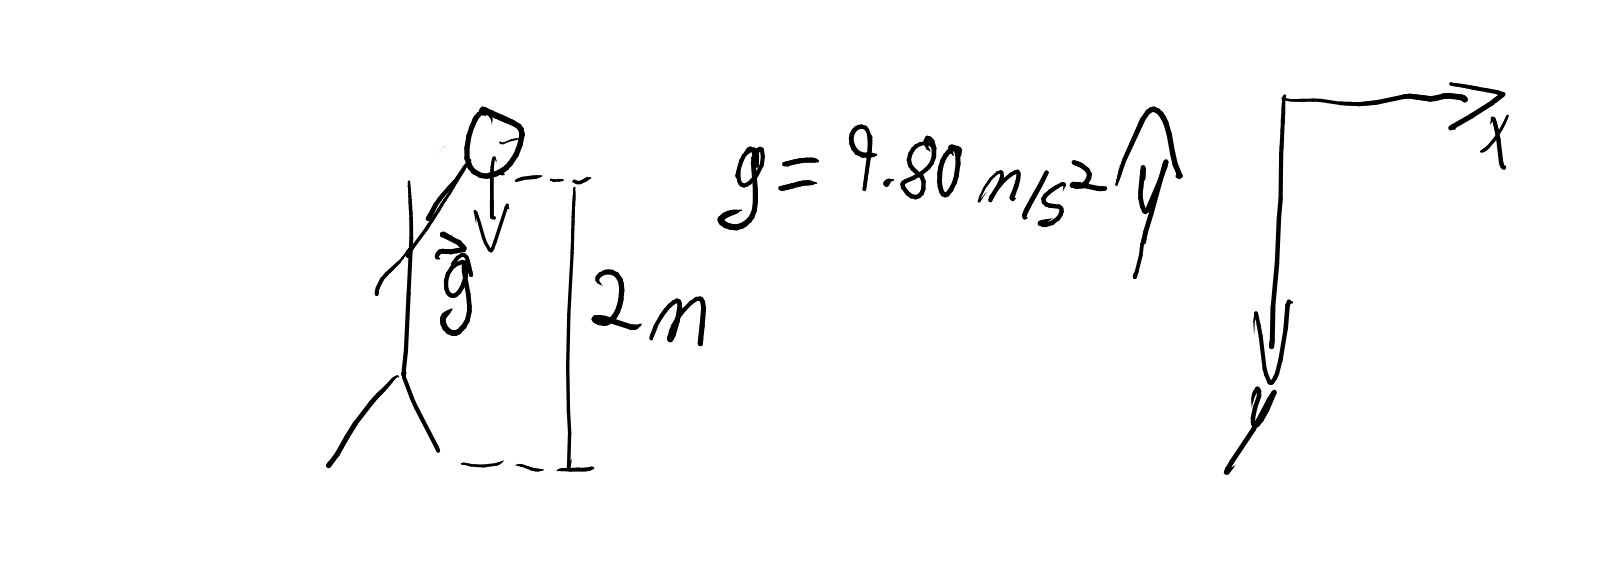
\includegraphics[scale=0.2]{energy_gravity.png}
\end{figure}

\parbox[][6cm][t]{8cm}{}

How about let's find the kinetic energy now. What is the speed of the ball when it hits the ground?

\parbox[][6cm][t]{8cm}{}

How long does it take the ball to hit the ground? (Recall $d=v_0t + \frac{1}{2}at^2$)

\parbox[][6cm][t]{8cm}{}

Finally, what is the kinetic energy of the ball when it hits the ground? Anything interesting?

\parbox[][10cm][t]{8cm}{}

\subsubsection{Spring}
There is energy stored in a spring as you compress it, and that is another form of potential energy. The equation needed to calculate this type of energy is $PE = \frac{1}{2}kx^{2}$. Where $k = 4.5 \times 10^3 \frac{N}{m^2}$ is called the spring constant, $PE$ is the potential energy, and $x$ is the displacement from the rest position. Suppose a spring has a spring constant of $k = 4.5 \times 10^3 \frac{N}{m}$, and is displaced by $0.5 m$ how fast will a $1kg$ ball, that was on top of the spring, be going after the spring is released and allowed to go to its rest position?

Please see the diagram below for an easier view of the problem. Keep in mind that according to conservation of energy $PE_{initial} + T_{initial} = PE_{final} + T_{final}$. From the problem there is no kinetic energy at the start, and no potential energy at the end. Have fun!

\begin{figure}[h]
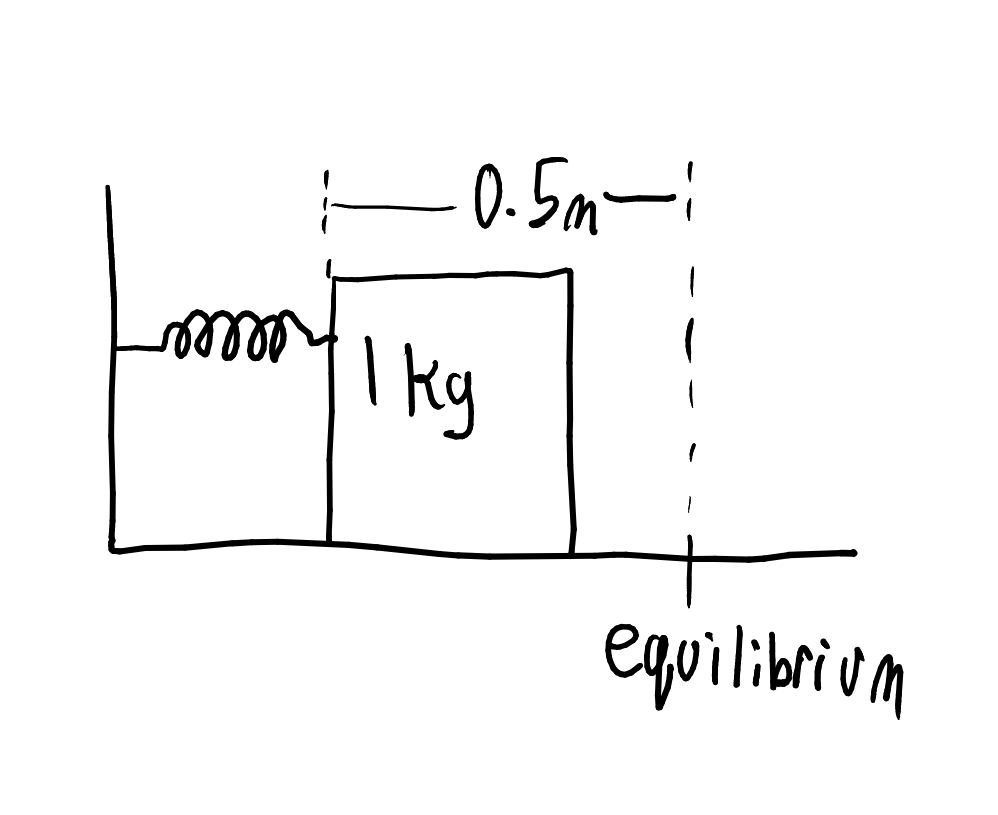
\includegraphics[scale=0.25]{energy_spring.png}
\end{figure}

\parbox[][10cm][t]{8cm}{}

\section{Friction}
Consider a block that weighs $5kg$ like the one shown below. In the diagram $F_{app}$ is the applied force but it is not used in this example.

\begin{figure}[h]
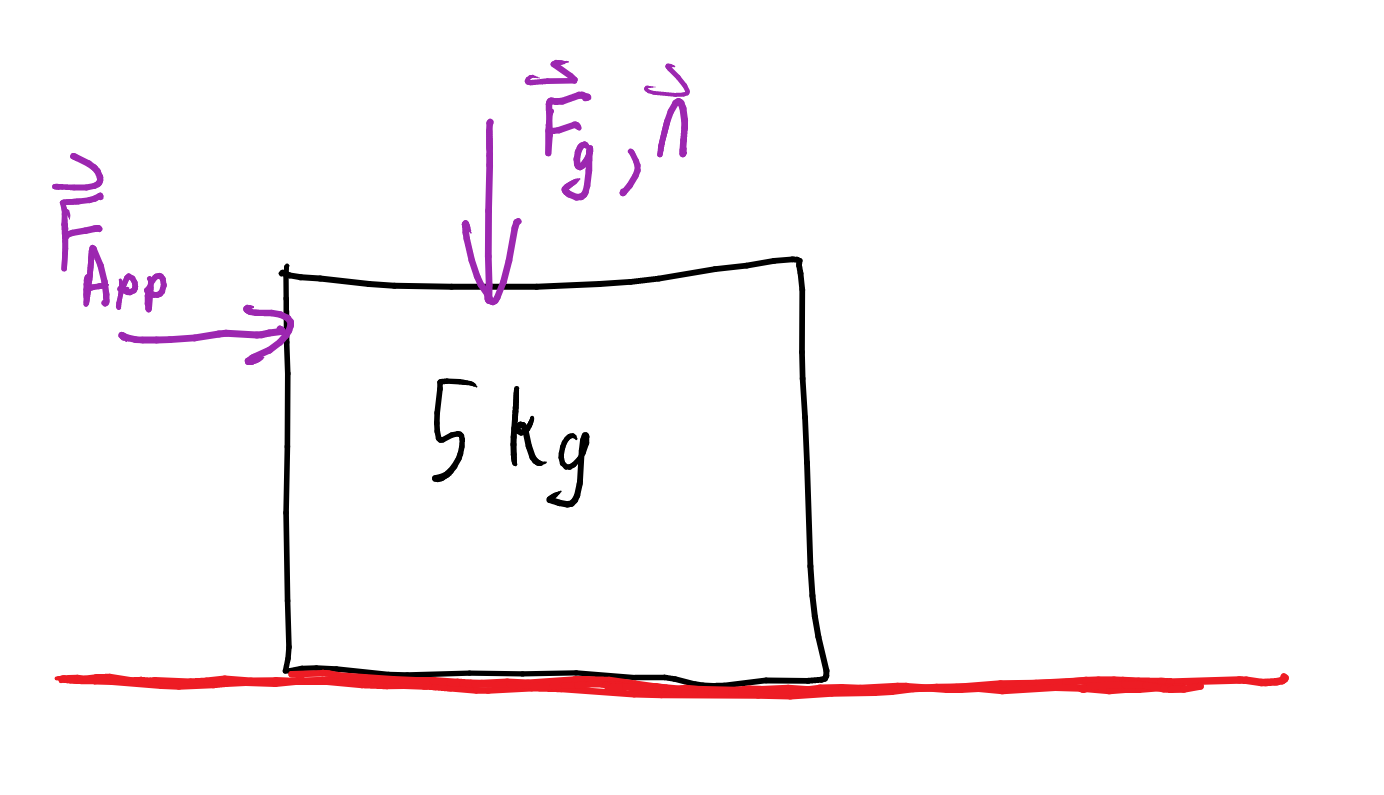
\includegraphics[scale=0.25]{energy_friction.png}
\end{figure}

What is $F_g$ (the force due to gravity)?

\parbox[][10cm][t]{8cm}{}

Now that we have the force due to gravity we can figure out the force of friction on the block as it is in motion. The equation for the force of friction is $f_{friction} = (\mu_k) * n$. Where $n = F_g$ or the force that is normal to the plane of motion, and $(\mu_k) = 0.5$ is called the coefficient of friction. What is the force of friction while someone is pushing the block?

\parbox[][10cm][t]{8cm}{}

 Finally use the equation from before that relates force distance and work to find out how much work is done just to overcome the force of friction moving $10m$

\parbox[][10cm][t]{8cm}{}


% \subsection{Bye bye dinasaors}
% Consider an asteroid that weighs $1.0 \times 10^16 kg$ assuming it starts at a velocity of
% make a separate worksheet

\begin{flushleft}
    \copyright  2020 Kody Rogers - kodyrogers21@gmail.com.

    This work is is licensed under a Creative Commons Attribution 4.0 International License.

    \url{https://creativecommons.org/licenses/by/4.0/}.
\end{flushleft}

%Above is the Discussion
%%%%%%%%%%%%%%%%%%%%%%%%%%%%%%%%%%%%%%%%%%%%%%%%%%%%%%%
\end{document}
